
\subsection{Test with $M=N$ on EEG Data Set}

\begin{figure}[H]
    \centering
	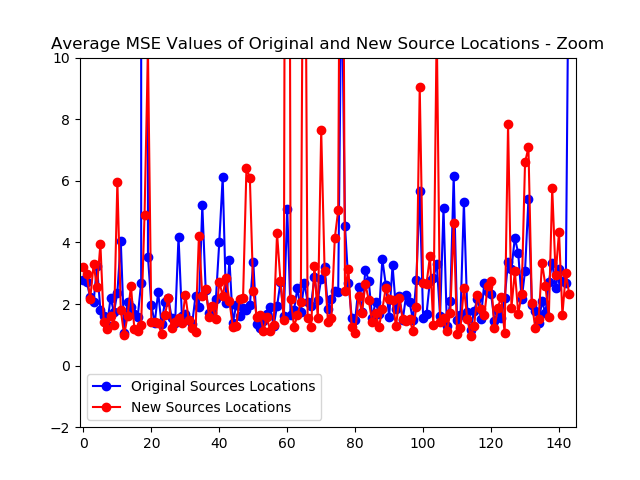
\includegraphics[scale=0.5]{figures/ch_7/M=N_1.png}
	\caption{Visualization of $\text{MSE}(\mathbf{X}, \hat{\mathbf{X}})$ of the main algorithm with simulated stochastic data sets specified by $M = 8$, $L=1000$ and $k = N$ for $N = M+1, \hdots , 36$. Average over 500 repetitions for each $N$.}
	\label{fig:varyN2}
\end{figure}  



\subsection{Test with $\frac{1}{3} M<N$ on EEG Data Set}

\subsection{Test with $\frac{1}{2} M<N$ on EEG Data Set}
